\section{Results}

We now evaluate the performance of NPRR, PostgreSQL and an in-memory triangle counting baseline. We release all the source codes of the algorithms used in our evaluation in \url{https://github.com/fabuzaid21/nprr}.


\subsection{Choice of Datasets} 

We used four large real-world datasets, which are from four different domains as shown in Table~\ref{datasets}. Facebook consists of `circles' (or `friends lists') from Facebook. Gnutella is a sequence of snapshots of the Gnutella peer-to-peer file sharing network from August 2002. Wikivote consists of votes deciding who is going to  be promoted as adminship. Condmat (Condense Matter Physics) collaboration network covers scientific collaborations between authors papers submitted to Condense Matter category. 


\begin{table}[!h]
\centering

\begin{tabular}{l|l|l}
Data & $|V|$ & $|E|$ \\
\hline
facebook & 4039 & 88234  \\
\hline
gnutella & 36682 & 88328 \\
\hline
wikivote & 7115 & 103689 \\
\hline
condmat & 23133 & 93479 \\
\hline
\end{tabular}
\caption{Datasets}
\label{datasets}
\end{table}



\subsection{Experimental Settings} 

We ran our experiments on a machine with a 2.4GHz Intel(R) Core(R) i5-4258U CPU and 8 GB DDR3-1,6000 RAM, running 64-bit MacOSX 10.11.2. NPRR was compiled with clang-700.1.81(Apple LLVM version 7.0.2). The optimization flag O2 option was enabled. PostgreSQL 9.4.5 was used during evaluation. All running time reported is the wall-clock time elapsed during computing.

\begin{figure}[!h]
    \centering
    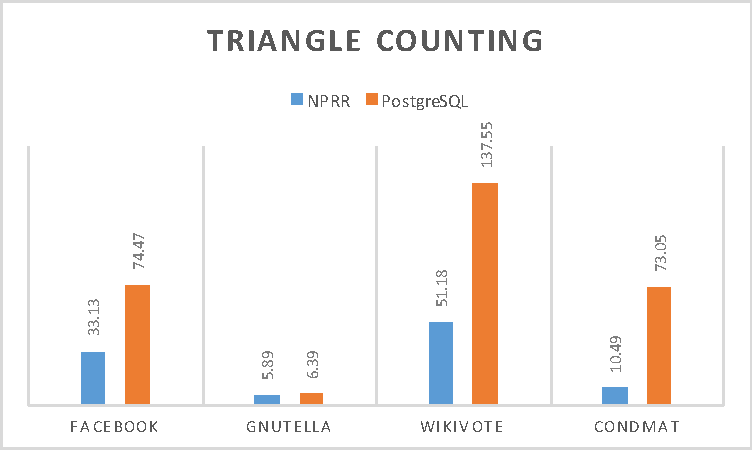
\includegraphics[width=0.8\columnwidth]{perf.pdf}
    \caption{Performance of NPRR and PostgreSQL}
    \label{perf}
\end{figure}

Figure~\ref{perf} shows the performance of NPRR and PostgreSQL on facebook, gnutella, wikivote and condmat. On gnutella, the performance of PostgreSQL is comparable to NPRR. On facebook, wikivote and condmat, the NPRR is about 2 - 6 times faster than PostgreSQL. 


\subsection{Native implementation}

We also provide a native high optimized implementation for triangle counting in C++. Interested readers can find the code in Appendix~\ref{native}.

\begin{figure}[!h]
    \centering
    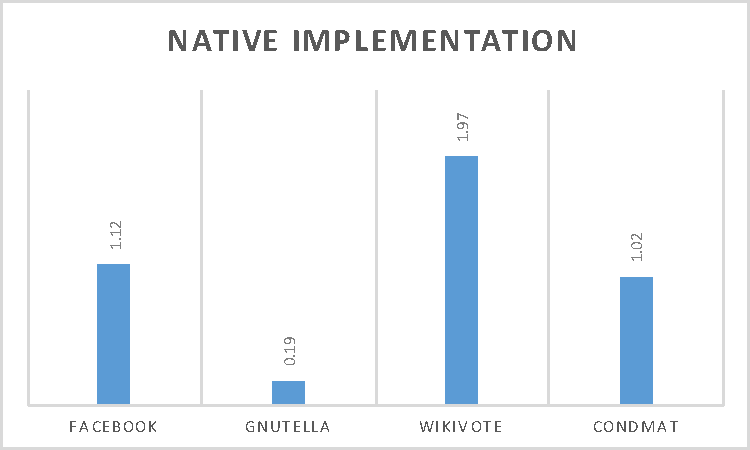
\includegraphics[width=0.8\columnwidth]{nativeperf.pdf}
    \caption{Performance of highly optimized native implementation}
    \label{nativeperf}
\end{figure}


Figure~\ref{nativeperf} shows the performance of our highly optimized native implementation on facebook, gnutella, wikivote and condmat. This provides a very clear reference point that shows the limit of performance. Our native implementation is about 10 - 25 times faster than NPRR. 
\subsection{Discussion}

We see the following key inferences: (1) Native code, as expected, delivers best performance since it is highly optimized for triangle counting. (2) NPRR performs better than PostgreSQL.
